\chapter{Studio del moto}

\section{Cinematica}

\subsection{Cinematica diretta}
\graphicspath{{media/2_kin_din/1_cin_dir}}

La cinematica diretta del robot SCARA è la seguente:
\[
\begin{cases}
    x = l_1 cos(\alpha)+l_2 cos(\alpha+\beta)\\
    y = l_1 sin(\alpha)+l_2 sin(\alpha+\beta)\\
    z = h - s\\
    g = \alpha+\beta+\gamma.
\end{cases}\]

dove la posa è costituita dalla terna $(x,y,z)$ che definisce le coordinate del gripper nel sistema di riferimento assoluto, mentre $g$ l'orientamento del gripper rispetto al semiasse positivo $x$.

La cinematica diretta è stata valutata utilizzando una MATLAB function apposita, che si riporta qua sotto.

\lstinputlisting[language=Octave]{media/1_intro/SCARAdir.m}

Si riporta di seguito lo script implementato per la simulazione della cinematica diretta del manipolatore SCARA.

\lstinputlisting[language=Octave, lastline=12]{media/2_kin_din/1_cin_dir/cinematica_SCARA_jac_dir.m}

La simulazione è stata svolta tra le coordinate definite ai giunti $Q_i = \begin{bmatrix}
    -0.5 & 0.1 & 0.1 & 0\\
\end{bmatrix}^{T}$ come punto iniziale della traiettoria e $Q_f = \begin{bmatrix}
    2 & 1 & 0.4 & -pi/4\\
\end{bmatrix}^{T}$ come punto finale. Queste coordinate, insieme alle caratteristiche geometriche e dinamiche del robot, sono state calcolate con i rispettivi script.

\lstinputlisting[language=Octave, firstline=13, lastline=35, firstnumber=13]{media/2_kin_din/1_cin_dir/cinematica_SCARA_jac_dir.m}

La legge di moto scelta è di tipo cicloidale, con una durata di 5 $s$, ed è stata calcolata separatamente per ciascuna coordinata ai giunti. Per ogni punto della traiettoria si è poi calcolata la posizione, velocità a accelerazioni assoluta attraverso l'uso dello jacobiano e della derivata dello jacobiano rispetto al tempo.

%\lstinputlisting[language=Octave, firstline=37, firstnumber=37]{media/2_kin_din/1_cin_dir/cinematica_SCARA_jac_dir.m}

Infine si esegue il plot dei grafici ottenuti. I risultati sono riportati nella figura \ref{fig:posa_dir_cin}.

\begin{figure}[H]
    \centering
    
\includegraphics[width=\linewidth]{posa}
    \caption{Posa e traiettoria compiuta dal manipolatore nella simulazione con traiettoria curvilinea.}
    \label{fig:posa_dir_cin}
\end{figure}

\begin{figure}[H]
    \centering
    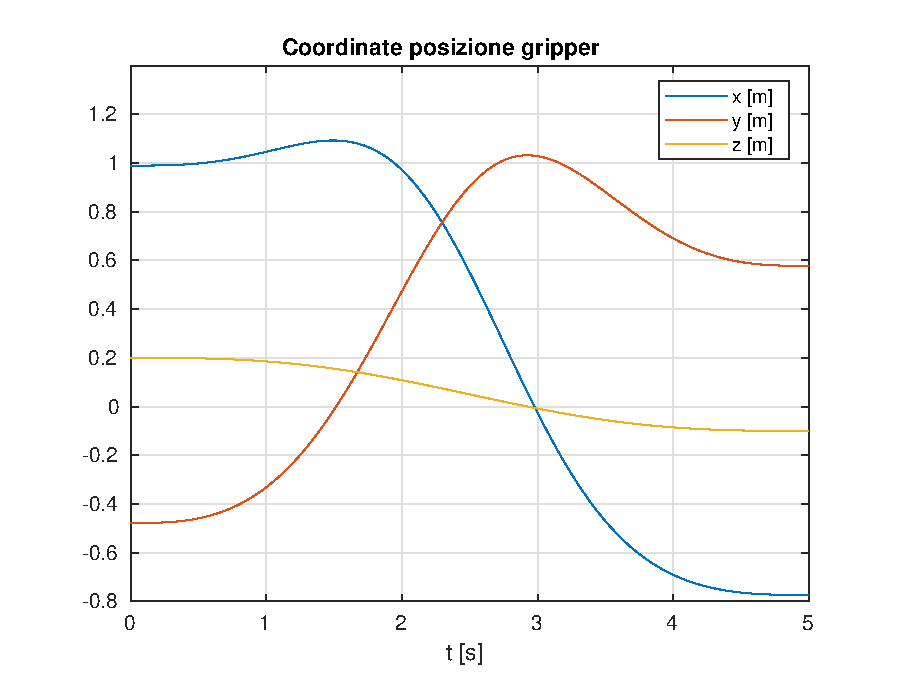
\includegraphics[width=0.7\linewidth]{posizione_gripper}
    \caption{Posizioni del gripper nel calcolo della cinematica diretta.}
    \label{fig:pos_gripper_dir_cin}
\end{figure}

\begin{figure}[H]
    \centering
    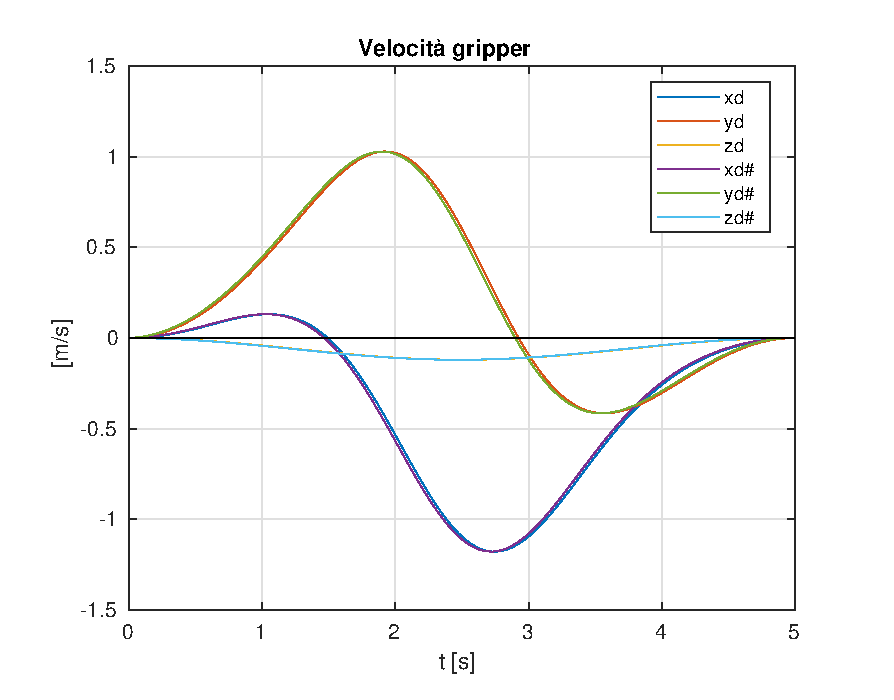
\includegraphics[width=0.7\linewidth]{velocità_gripper}
    \caption{Velocità del gripper nel calcolo della cinematica diretta. Le grandezze che terminano con $\#$ sono state ricavate tramite derivazione alle differenze finite delle rispettive coordinate di posizione.}
    \label{fig:vel_gripper_dir_cin}
\end{figure}

\begin{figure}[H]
    \centering
    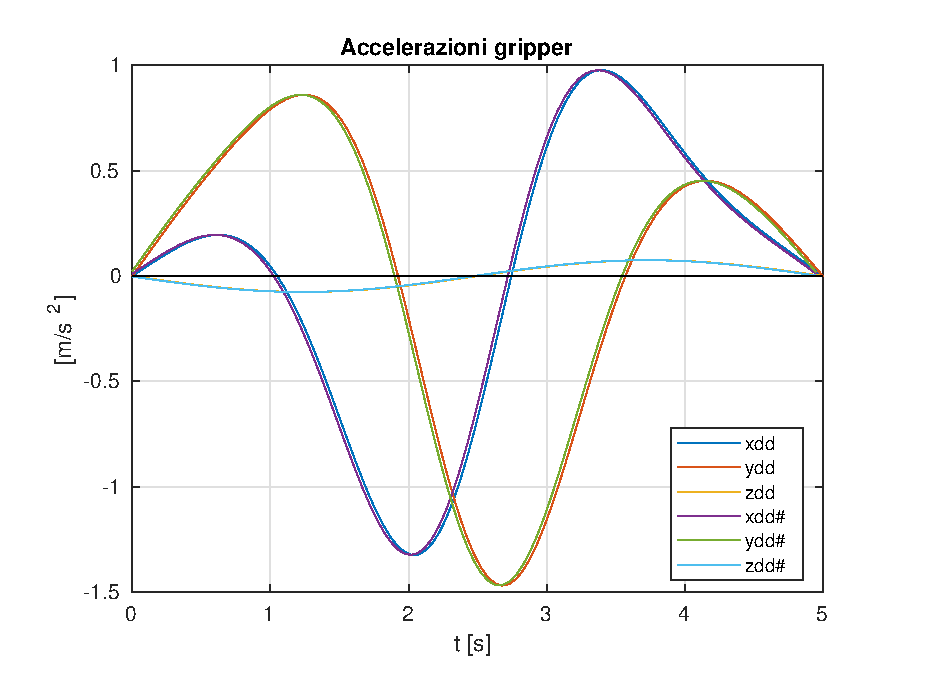
\includegraphics[width=0.7\linewidth]{accelerazione_gripper}
    \caption{Accelerazioni del gripper nel calcolo della cinematica diretta. Le grandezze che terminano con $\#$ sono state ricavate tramite derivazione alle differenze finite delle rispettive velocità.}
    \label{fig:acc_gripper_dir_cin}
\end{figure}

\begin{figure}[H]
    \centering
    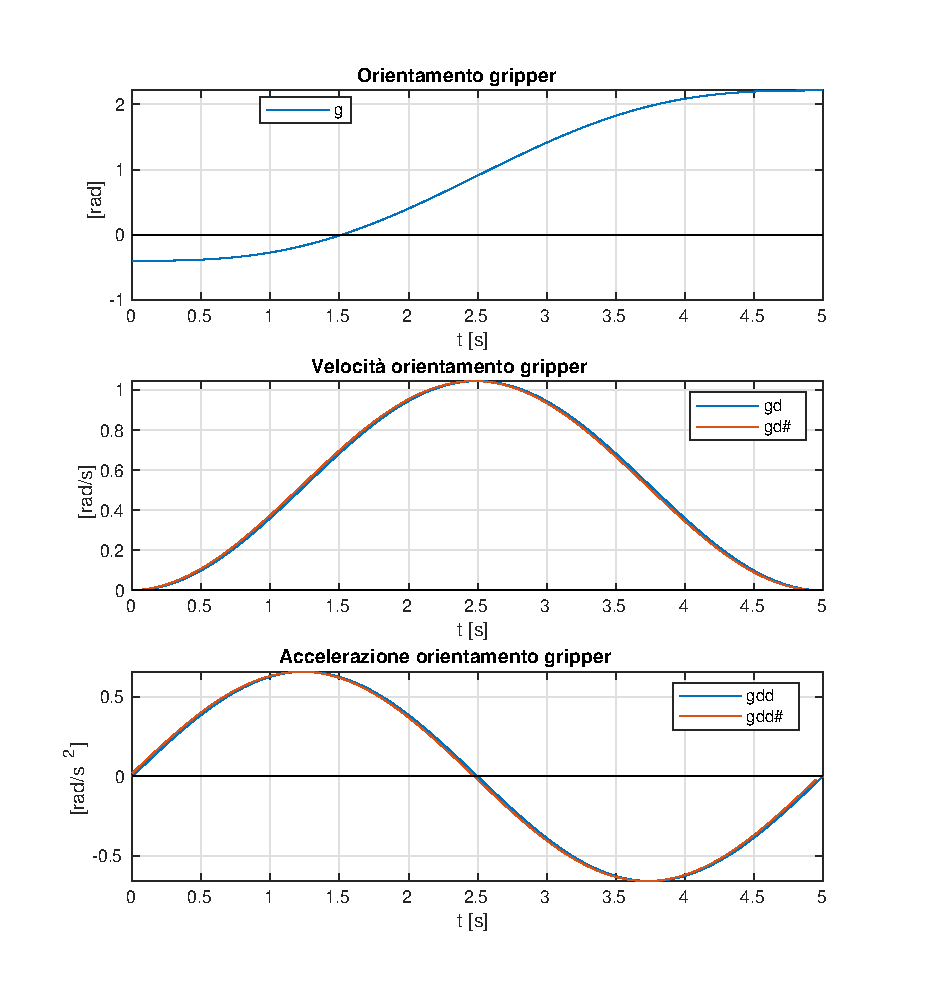
\includegraphics[width=0.7\linewidth]{g_joint}
    \caption{Coordinate di orientamento, velocità ed accelerazione del quarto giunto rotoidale (gripper). Le grandezze che terminano con $\#$ sono state ricavate tramite derivazione alle differenze finite delle rispettive posizioni e velocità.}
    \label{fig:gripper_dir_cin}
\end{figure}


\subsection{Cinematica inversa}
\graphicspath{{media/2_kin_din/2_cin_inv}}

La cinematica inversa del robot SCARA è la seguente:

\[
\begin{cases}
	\alpha=atan(\frac{y}{x})-atan(\frac{l_2sin(q_2)}{l_1+l_2cos(q_2)})\\
	\beta=\pm acos(\frac{(x^2+y^2-l_1^2-l_2^2)}{(2l_1l_2)})\\
	s=h-z\\
	\gamma=g-\alpha-\beta\\
\end{cases}\].

La cinematica inversa è stata calcolata per via analitica con la funzione riportata in seguito. Per il giunto \beta si è scelto arbitrariamente la configurazione $ \beta=+acos(\frac{(x^2+y^2-l_1^2-l_2^2)}{(2l_1l_2)}) $ positiva.

\lstinputlisting[language=Octave]{media/2_kin_din/2_cin_inv/SCARAinvAnalitica.m}

Si riporta in seguito la simulazione della traiettoria, definita rispetto al sistema di riferimento posto alla base del robot, tra il punto di coordinate  $S_i = \begin{bmatrix}
     -0.9 & 0.4 & 0 & 0 \\
\end{bmatrix}^{T}$ al punto $S_f = \begin{bmatrix}
     0.7 & 0.2 & 0.1 & \frac{\pi}{3} \\
\end{bmatrix}^{T}$.

\lstinputlisting[language=Octave,lastline=38]{media/2_kin_din/2_cin_inv/cinematica_SCARA_jac_inv.m}

Si riportano di seguito i risultati della simulazione sia nello spazio di lavoro che ai giunti.

\begin{figure}[H]
    \centering
    
\includegraphics[width=\linewidth]{posa}
    \caption{Posa e traiettoria compiuta dal manipolatore nella simulazione con traiettoria rettilinea.}
    \label{fig:enter-label}
\end{figure}

\begin{figure}[H]
    \centering
    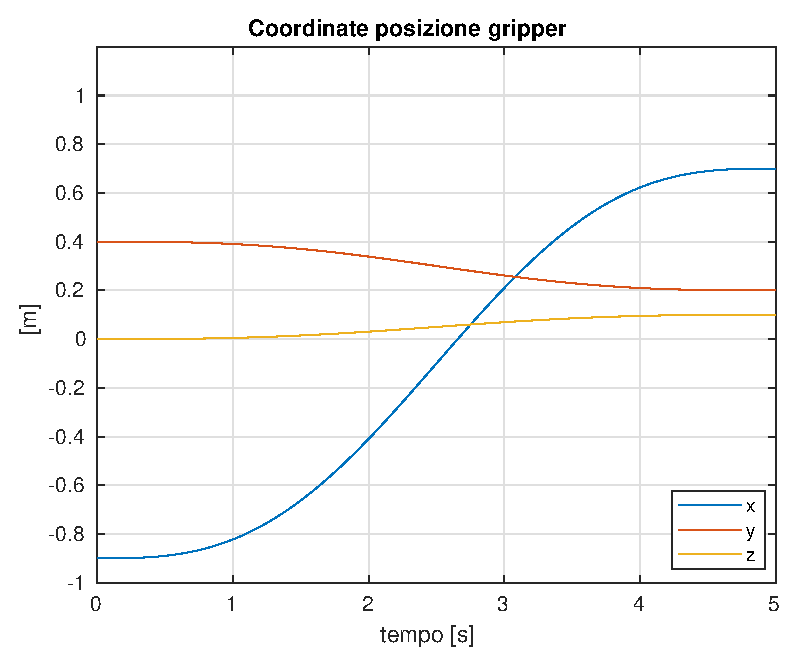
\includegraphics[width=0.65\linewidth]{pos_fisso.eps}
    \caption{Posizione del gripper nel sistema di riferimento alla base del robot.}
    \label{fig:enter-label}
\end{figure}

\begin{figure}[H]
    \centering
    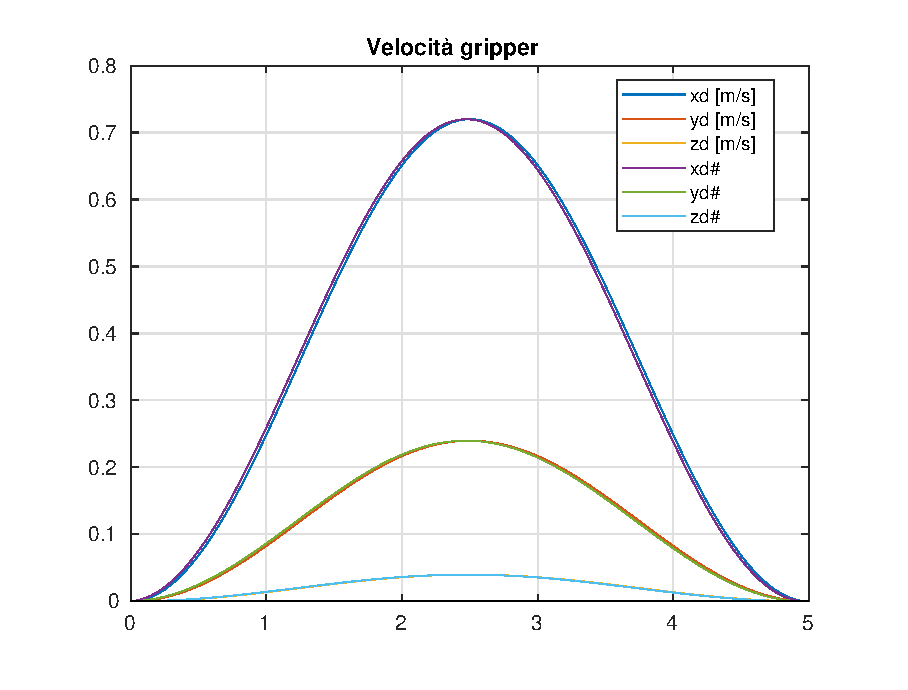
\includegraphics[width=0.65\linewidth]{vel_fisso}
    \caption{Velocità del gripper nel sistema di riferimento alla base del robot. Le grandezze che terminano con $\#$ sono state ricavate tramite derivazione alle differenze finite delle rispettive velocità.}
    \label{fig:enter-label}
\end{figure}

\begin{figure}[H]
    \centering
    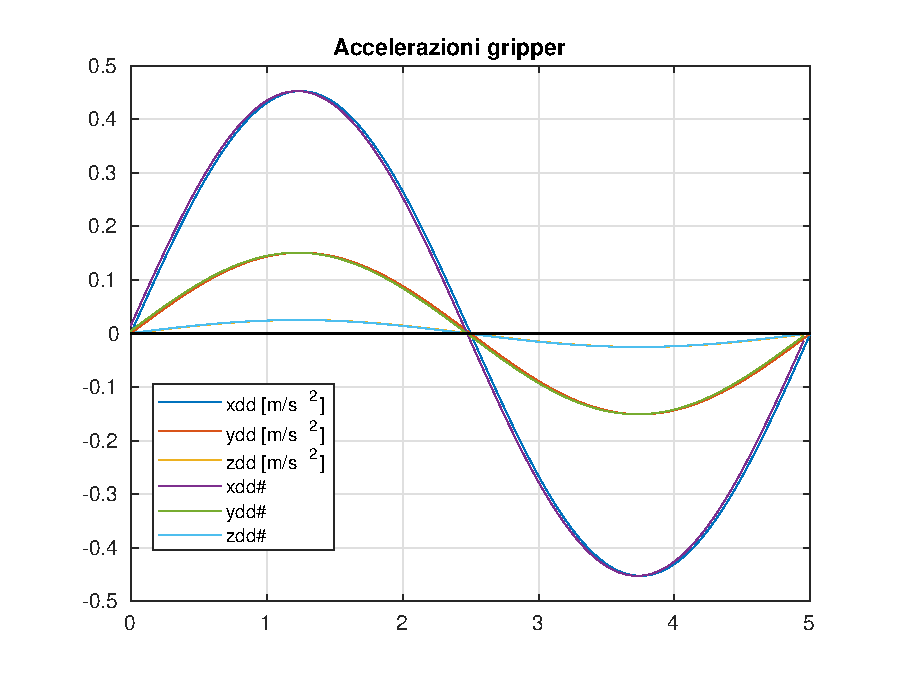
\includegraphics[width=0.65\linewidth]{acc_fisso}
    \caption{Accelerazione del gripper nel sistema di riferimento alla base del robot. Le grandezze che terminano con $\#$ sono state ricavate tramite derivazione alle differenze finite delle rispettive velocità.}
    \label{fig:enter-label}
\end{figure}

\begin{figure}[H]
    \centering
    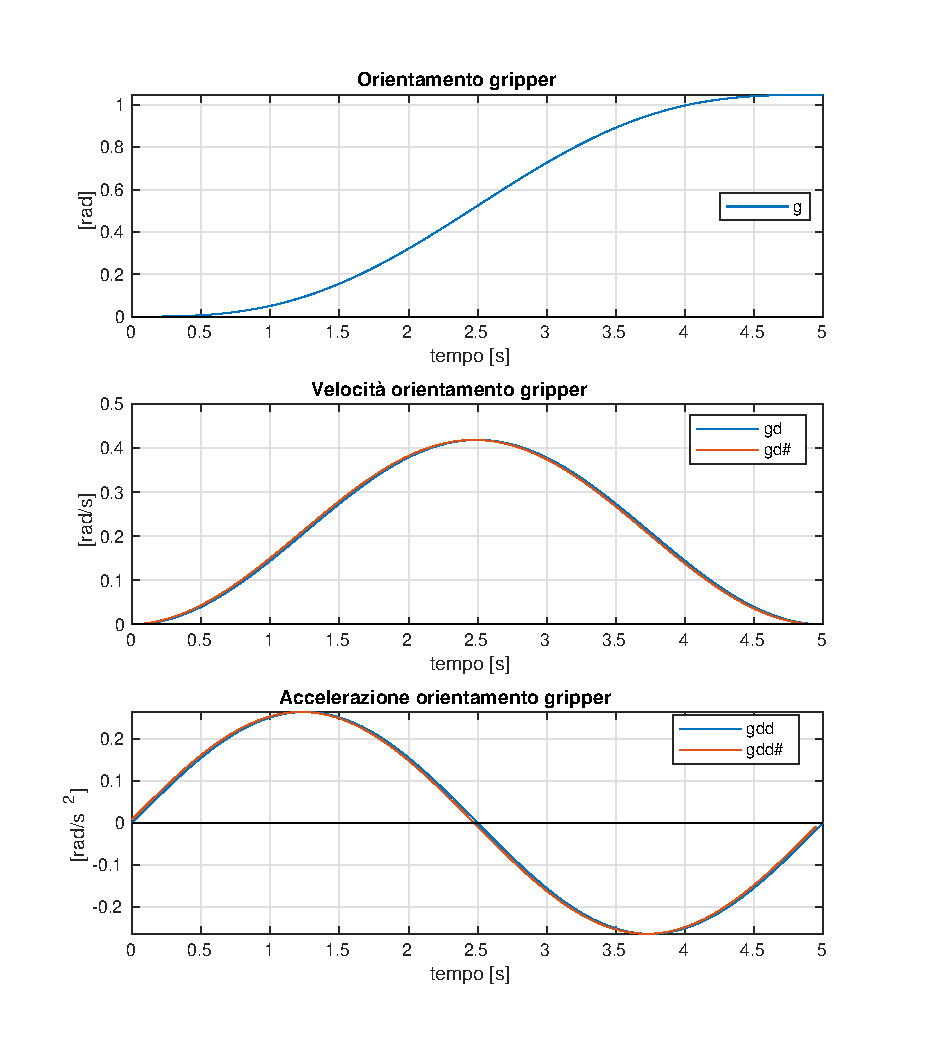
\includegraphics[width=0.7\linewidth]{gripper_fisso}
    \caption{Orientamento del gripper nel sistema di riferimento alla base del robot. Le grandezze che terminano con $\#$ sono state ricavate tramite derivazione alle differenze finite delle rispettive velocità.}
    \label{fig:enter-label}
\end{figure}

\begin{figure}[H]
    \centering
    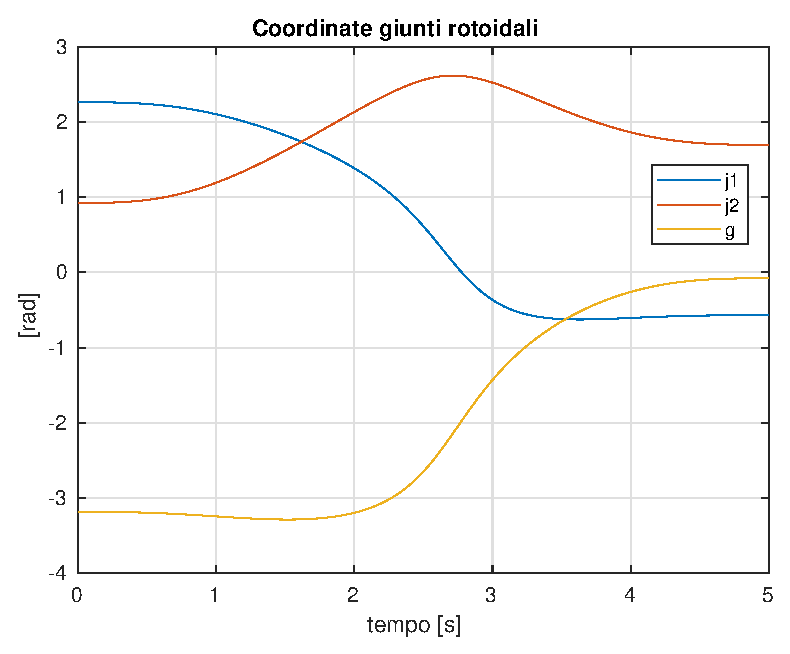
\includegraphics[width=0.65\textwidth]{pos_giunti}
    \caption{Orientamento dei giunti durante la traiettoria simulata.}
    \label{fig:enter-label}
\end{figure}

\begin{figure}[H]
    \centering
    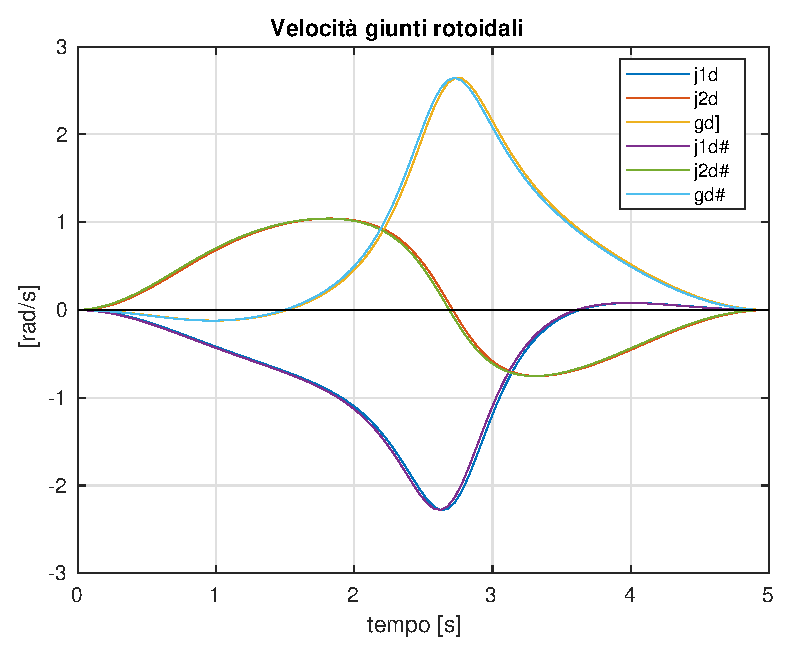
\includegraphics[width=0.65\textwidth]{vel_giunti}
    \caption{Velocità dei giunti durante la traiettoria simulata. Le grandezze che terminano con $\#$ sono state ricavate tramite derivazione alle differenze finite delle rispettive velocità.}
    \label{fig:enter-label}
\end{figure}

\begin{figure}[H]
    \centering
    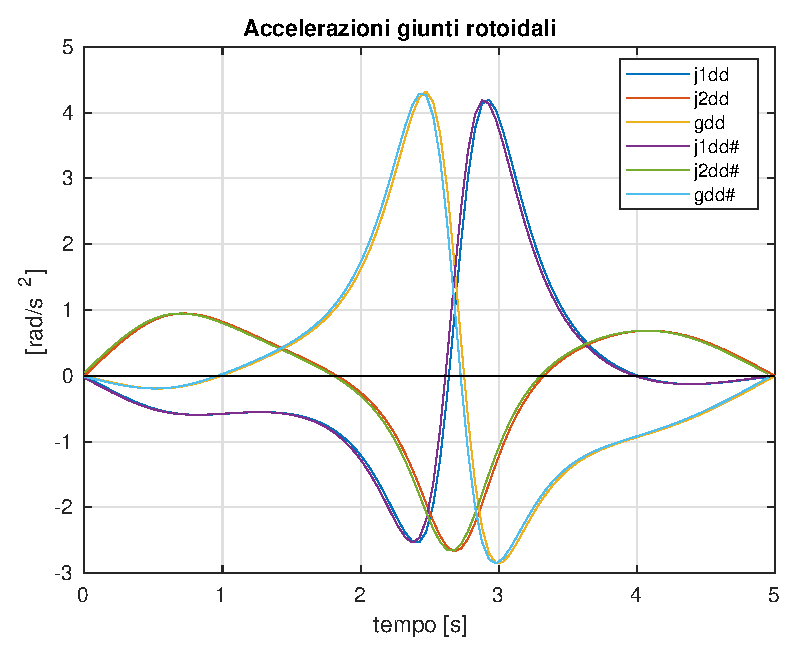
\includegraphics[width=0.65\linewidth]{acc_giunti}
    \caption{Accelerazione dei giunti durante la traiettoria simulata. Le grandezze che terminano con $\#$ sono state ricavate tramite derivazione alle differenze finite delle rispettive velocità.}
    \label{fig:enter-label}
\end{figure}

\begin{figure}[H]
    \centering
    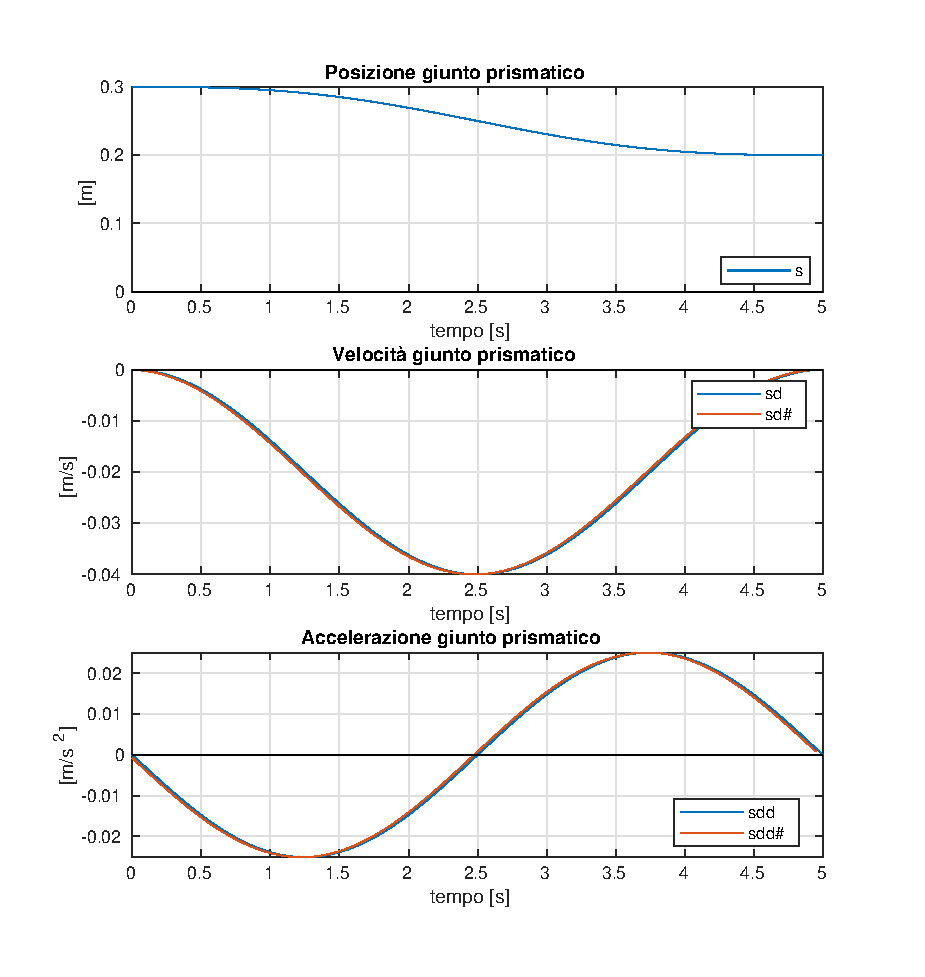
\includegraphics[width=0.7\linewidth]{prism_giunti}
    \caption{Posizione, velocità e accelerazione del giunto prismatico durante la traiettoria simulata. Le grandezze che terminano con $\#$ sono state ricavate tramite derivazione alle differenze finite delle rispettive velocità.}
    \label{fig:enter-label}
\end{figure}

\newpage
\section{Dinamica inversa},
\label{chapter:dinamica_inversa}
\graphicspath{{media/2_kin_din/3_din_inv}}

Le coppie e forze ai giunti del manipolatore sono state calcolate secondo il modello:
\[ F_{q} = \left( J_e^{T}MJ_e \right) \ddot{Q}+\left( J_e^{T}M\dot{J_e} \right) \dot{Q} -J_e^{T}F_{se} + J_e^{T} M A_g\]

\lstinputlisting[language=Octave,firstline=12,lastline=19,firstnumber=12]{media/2_kin_din/3_din_inv/dinamica_SCARA_jac_inv.m}

nel quale:
\begin{itemize}
	\item la cinematica estesa del manipolatore corrisponde alla seguente matrice 
	\[ S_e=
	\begin{bmatrix}
		x_4 = l_1cos(a)+l_2cos(\alpha+\beta)\\
		y_4 = l_1sin(\alpha)+l_2sin(\alpha+\beta)\\
		z_4 = h-s\\
		g_4 = \alpha+\beta+\gamma\\
		x_3 = l_1cos(\alpha)+l_2cos(\alpha+\beta)\\
		y_3 = l_1sin(\alpha)+l_2sin(\alpha+\beta)\\
		z_3 = h-s+g_3\\
		x_2 = l_1cos(\alpha)+g_2cos(\alpha+\beta)\\
		y_2 = l_1sin(\alpha)+g_2sin(\alpha+\beta)\\
		z_2 = h\\
		g_2 = \alpha+\beta\\
		x_1 = g_1cos(\alpha)\\
		y_2 = g_1sin(\alpha)\\
		z_1 = h\\
		g_1 = \alpha.
	\end{bmatrix}
	\]
	\item lo Jacobiano esteso 
	\[  J_e =
	\begin{bmatrix}
		-l_1sin(\alpha)-l_2sin(\alpha+\beta) & -l_2sin(\alpha+\beta) & 0 & 0 \\
		l_1cos(\alpha)+l_2cos(\alpha+\beta) & l_2cos(\alpha+\beta) & 0 & 0\\
		0 & 0 & -1 & 0\\
		1 & 1 & 0 & 1\\
		-l_1sin(\alpha)-l_2sin(\alpha+\beta) & -l_2sin(\alpha+\beta) & 0 & 0\\
		l_1cos(\alpha)+l_2cos(\alpha+\beta) & l_2cos(\alpha+\beta) & 0 & 0\\
		0 & 0 & -1 & 0\\
		-l_1sin(\alpha)-g_2sin(\alpha+\beta) & -g_2sin(\alpha+\beta) & 0 & 0\\
		l_1cos(\alpha)+g_2cos(\alpha+\beta) & g_2cos(\alpha+\beta) & 0 & 0\\
		0 & 0 & 0 & 0\\
		1 & 1 & 0 & 0\\
		-g_1sin(\alpha) & 0 & 0 & 0\\
		g_1cos(\alpha) & 0 & 0 & 0\\
		0 & 0 & 0 & 0\\
		1 & 0 & 0 & 0\\
	\end{bmatrix}
	\]
	\item mentre la derivata dello Jacobiano esteso 
	\[ \Dot{J_e} =
	\begin{bmatrix}
		-l_1cos(\alpha)\Dot{\alpha}-l_2cos(\alpha+\beta)(\Dot{\alpha}+\Dot{\beta}) & -l_2cos(\alpha+\beta)(\Dot{\alpha}+\Dot{\beta}) & 0 & 0\\
		-l_1sin(\alpha)\Dot{\alpha}-l_2sin(\alpha+\beta)(\Dot{\alpha}+\Dot{\beta}) & -l_2sin(\alpha+\beta)(\Dot{\alpha}+\Dot{\beta}) & 0 & 0\\
		0 & 0 & 0 & 0\\
		0 & 0 & 0 & 0\\
		-l_1cos(\alpha)\Dot{\alpha}-l_2cos(\alpha+\beta)(\Dot{\alpha}+\Dot{\beta}) & -l_2cos(\alpha+\beta)(\Dot{\alpha}+\Dot{\beta}) & 0 & 0\\
		-l_1sin(\alpha)\Dot{\alpha}-l_2sin(\alpha+\beta)(\Dot{\alpha}+\Dot{\beta}) & -l_2sin(\alpha+\beta)(\Dot{\alpha}+\Dot{\beta}) & 0 & 0\\
		0 & 0 & 0 & 0\\
		-l_1cos(\alpha)\Dot{\alpha}-g_2cos(\alpha+\beta)(\Dot{\alpha}+\Dot{\beta}) & -g_2cos(\alpha+\beta)(\Dot{\alpha}+\Dot{\beta}) & 0 & 0\\
		-l_1sin(\alpha)\Dot{\alpha}-g_2sin(\alpha+\beta)(\Dot{\alpha}+\Dot{\beta}) & -g_2sin(\alpha+\beta)(\Dot{\alpha}+\Dot{\beta}) & 0 & 0\\
		0 & 0 & 0 & 0\\
		0 & 0 & 0 & 0\\
		-g_1cos(\alpha)\Dot{\alpha} & 0 & 0 & 0\\
		-g_1sin(\alpha)\Dot{\alpha} & 0 & 0 & 0\\
		0 & 0 & 0 & 0\\
		0 & 0 & 0 & 0\\
	\end{bmatrix}
	\]
\end{itemize} 


La dinamica è stata controllata calcolando l'energia totale, come somma dell'energia potenziale e cinetica, e confrontando la derivata prima dell'energia totale con la potenza assorbita dai giunti del manipolatore. 

\lstinputlisting[language=Octave,firstline=42,lastline=76,firstnumber=42]{media/2_kin_din/3_din_inv/dinamica_SCARA_jac_inv.m}

L'energia cinetica è stata calcolata come \[ E_k = \frac{1}{2}\dot{Q}^{T} J_e^{T}MJ_e\dot{Q}\]

L'energia potenziale è stata calcolata come \[ E_p = S_e^{T}MA_g+E_{e_{0}}\]

La potenza assorbita dai giunti è stata calcolata come \[ W = F_q^{T}\dot{Q}+F_{se}^{T}\dot{S_e}\]

Di seguito si riportano i risultati del calcolo della dinamica inversa.

\begin{figure}[htpb!]
	\centering
	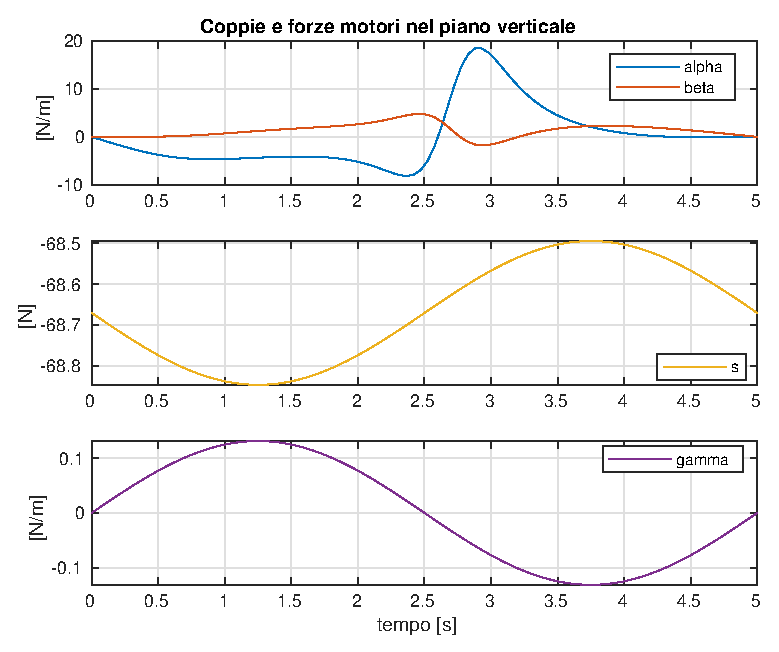
\includegraphics[width=0.7\linewidth]{media/2_kin_din/3_din_inv/coppie}
	\caption{Coppie e forze della traiettoria simulata.}
	\label{fig:coppie}
\end{figure}

\begin{figure}[htpb!]
	\centering
	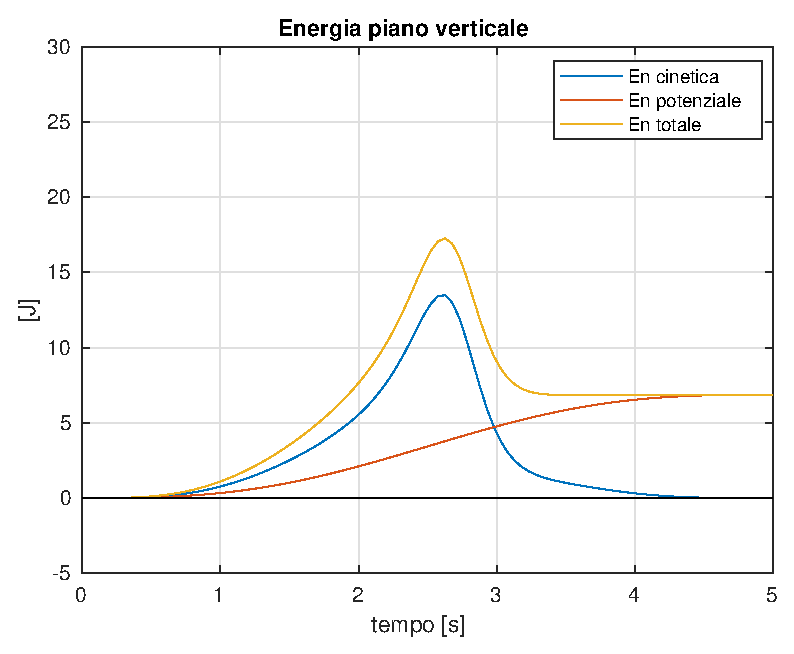
\includegraphics[width=0.7\linewidth]{media/2_kin_din/3_din_inv/energia}
	\caption{Energia assorbita dai giunti nella traiettoria simulata.}
	\label{fig:energia}
\end{figure}

\begin{figure}[htpb!]
	\centering
	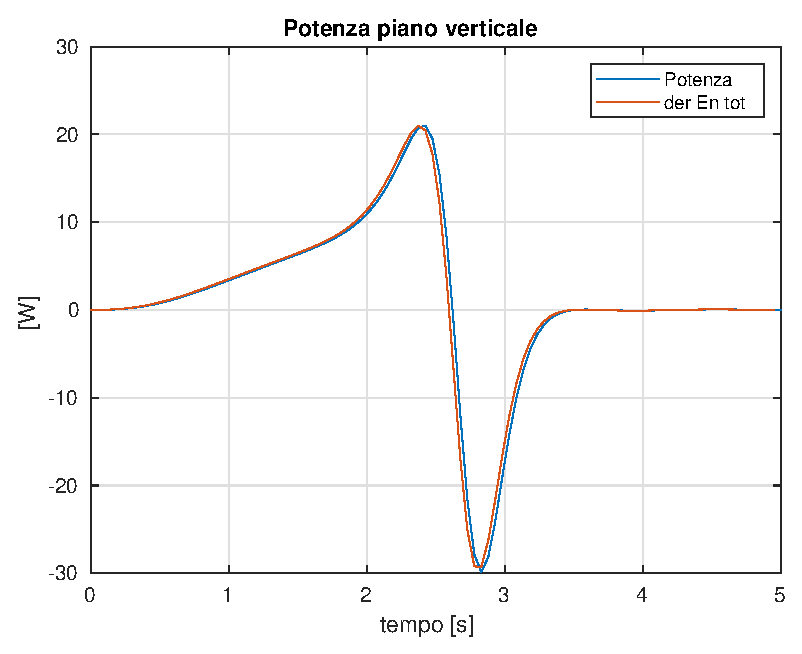
\includegraphics[width=0.7\linewidth]{media/2_kin_din/3_din_inv/potenza}
	\caption{Potenza assorbita dai giunti nella traiettoria simulata.}
	\label{fig:potenza}
\end{figure}

